%!TEX root = ../var.tex
На практике элементарные случайные события являются либо числами, либо наборами чисел (случайными векторами). В \S\S\ \ref{par:11}–\ref{par:13} мы изучим
одномерные случайные величины, у которых $\Omega\subset\mathbb{R}^1$ — числовое множество. Начиная с \S\ref{par:13} изучим случайные векторы, у которых  
$\Omega\subset\mathbb{R}^n$, при $n \geqslant 2$.

Дадим общее определение случайной величины. Пусть $(\Omega, \mathcal{A}, \mathcal{P})$ -- произвольное вероятностное пространство.

\begin{definition}
\label{def:11.1}
	Функция $\xi : \Omega \rightarrow \mathbb{R}$ называется случайной величиной на $\sigma$-алгебре событий $A$, если для любого числа $x\in\mathbb{R}$ прообраз луча
	$\xi^{-1}((-\infty,x])=\{\omega\in\Omega|\xi(\omega)\leqslant x\}$
	 является событием из $\sigma$-алгебры $\mathfrak{A}$.
\end{definition}

\begin{zam}
\label{zam:11.2}
	
1) Самая простая функция $\xi : \Omega \rightarrow \mathbb{R}$ — это постоянная функция, заданная для любого $\omega \in \Omega$ по формуле $\xi(\omega)=c$. Она
принимает одно значение и является не случайной, а детерминированной.
Она рассматривается в теории вероятностей как частный тривиальный
случай.

2) Первая нетривиальная случайная величина (с $\Omega \in \mathbb{R}$) задаётся
с помощью тождественной функции $\xi(\omega) = \omega$. В этом случае событие
$\xi^{-1}((-\infty,x])=\{\omega\in\Omega|\xi(\omega)\leqslant x\}$ обозначают короче: $\{\xi \leqslant x\}$.

3) Оказывается, что другие случайные величины ($\xi(\omega) \neq \omega$) могут быть
описаны через случайную величину $\xi(\omega) = \omega$. Это будет показано в \S\ref{par:13}.
\end{zam}

\begin{definition}
\label{def:11.3}
	Функцией распределения случайной величины $\xi$ называется функция $F_{\xi}(x) : \mathbb{R} \rightarrow [0, 1]$, определённая по формуле
$$F_{\xi}(x)=\P(\xi\leqslant x)$$.
\end{definition}

Очевидно, что $0\leqslant F_{\xi}(x)\leqslant 1$

\begin{figure}[h!]
	\centering
	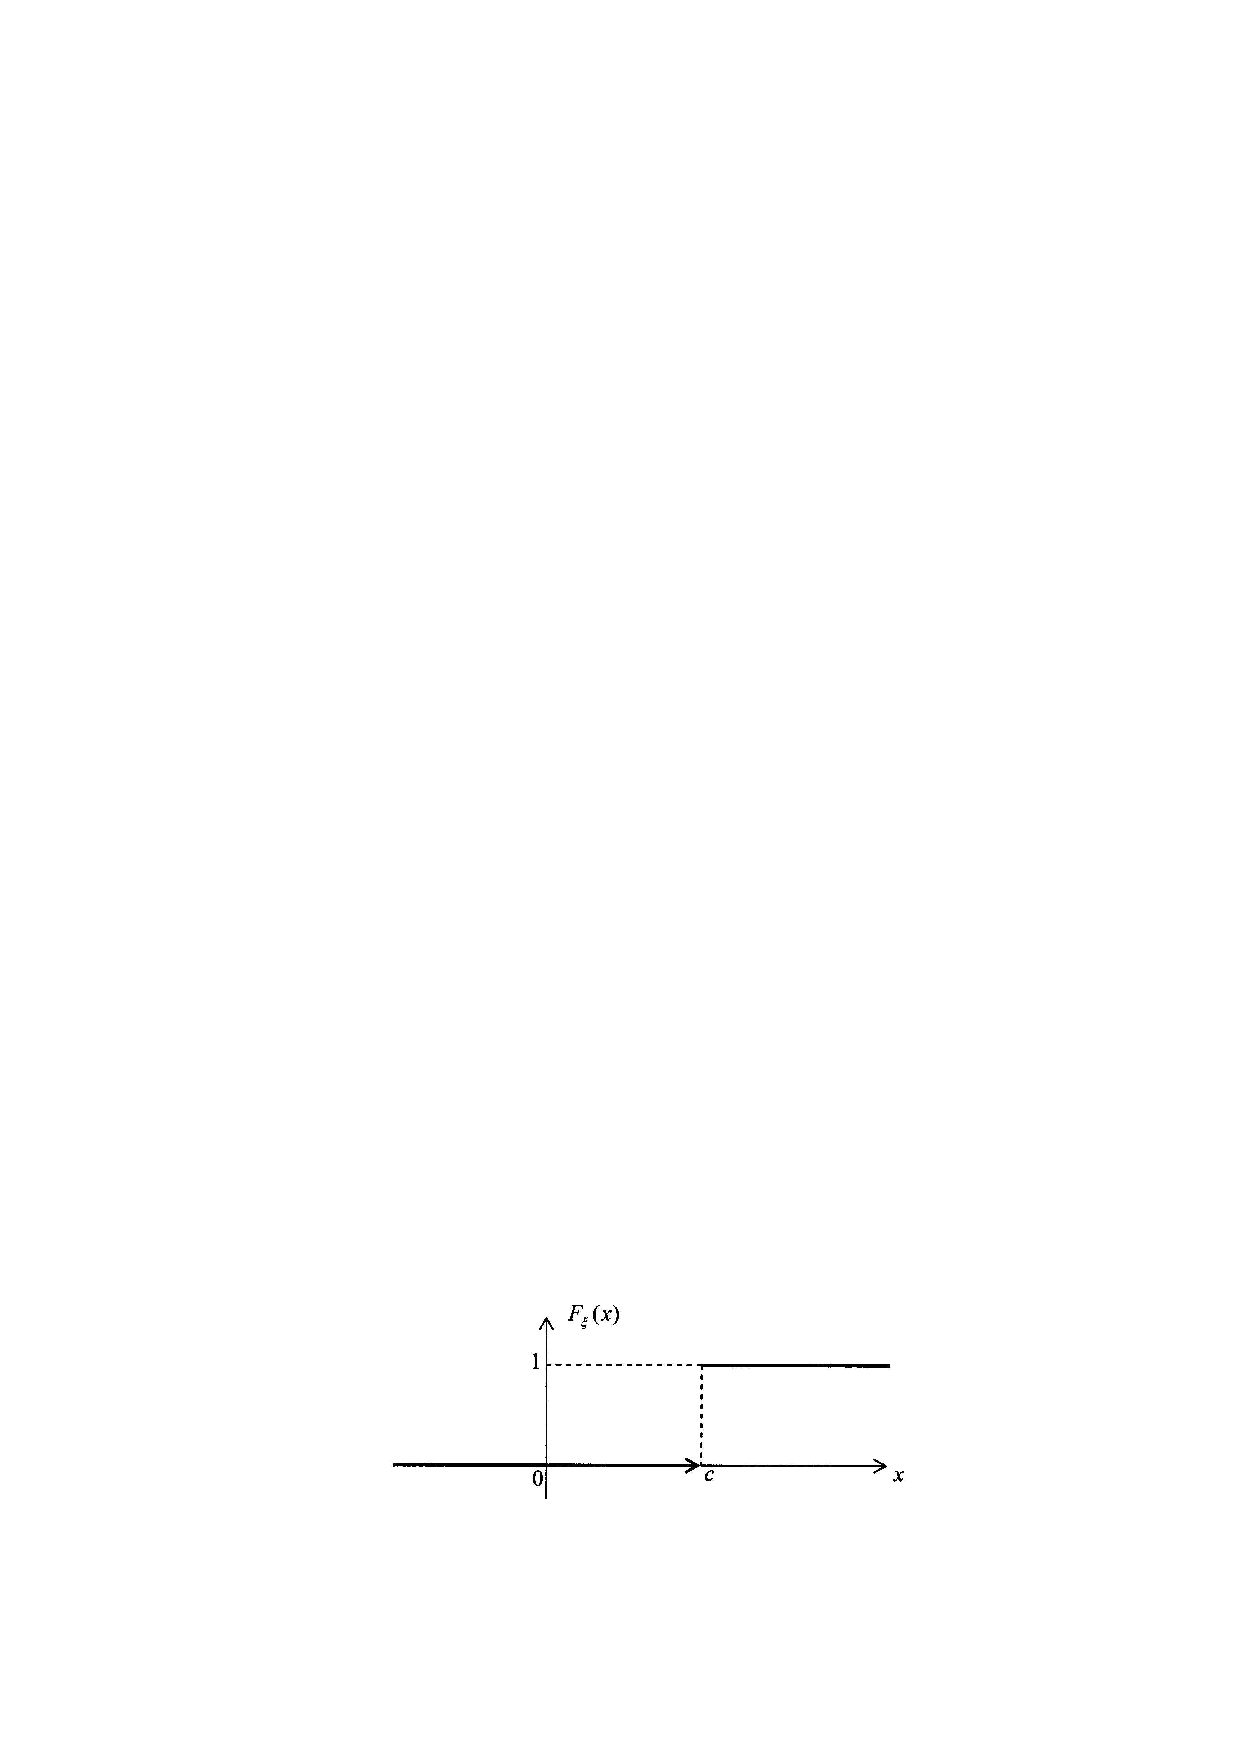
\includegraphics[]{pic/pic9}
	\caption{Функция распределения детерминированной величины.}
	\label{fig9}
\end{figure}

\textbf{Примеры}

	1) Детерминированная (вырожденная случайная) величина $\xi : \Omega \rightarrow \mathbb{R}$ имеет пространство элементарных событий, состоящее
из одного элементарного события, $\Omega = \{\omega\}$. Она принимает только одно
значение $\xi(\omega)=c=const\in\mathbb{R}$ с вероятностью равной 1, т.е. имеет ряд
распределения 
\begin{tabular}{|c|c|}
\hline
$\xi$ & $c$\\ \hline
$\P$ & $1$\\ \hline
\end{tabular}
. Её функция распределения показана на рис. \ref{fig9}.

2) Случайная величина $\xi$, имеющая распределение Бернулли, и принимающая значения 1 (успех) и 0 (неудача) с вероятностями соответственно
$p$ и $1 − p$, имеет ряд распределения 
\begin{tabular}{|c|c|c|}
\hline
$\xi$ & $0$ & $1$\\ \hline
$\P$   & $1-p$ & $p$\\ \hline
\end{tabular}
 и имеет график, показанный на рис. \ref{fig10}.



\begin{figure}[h!]
	\centering
	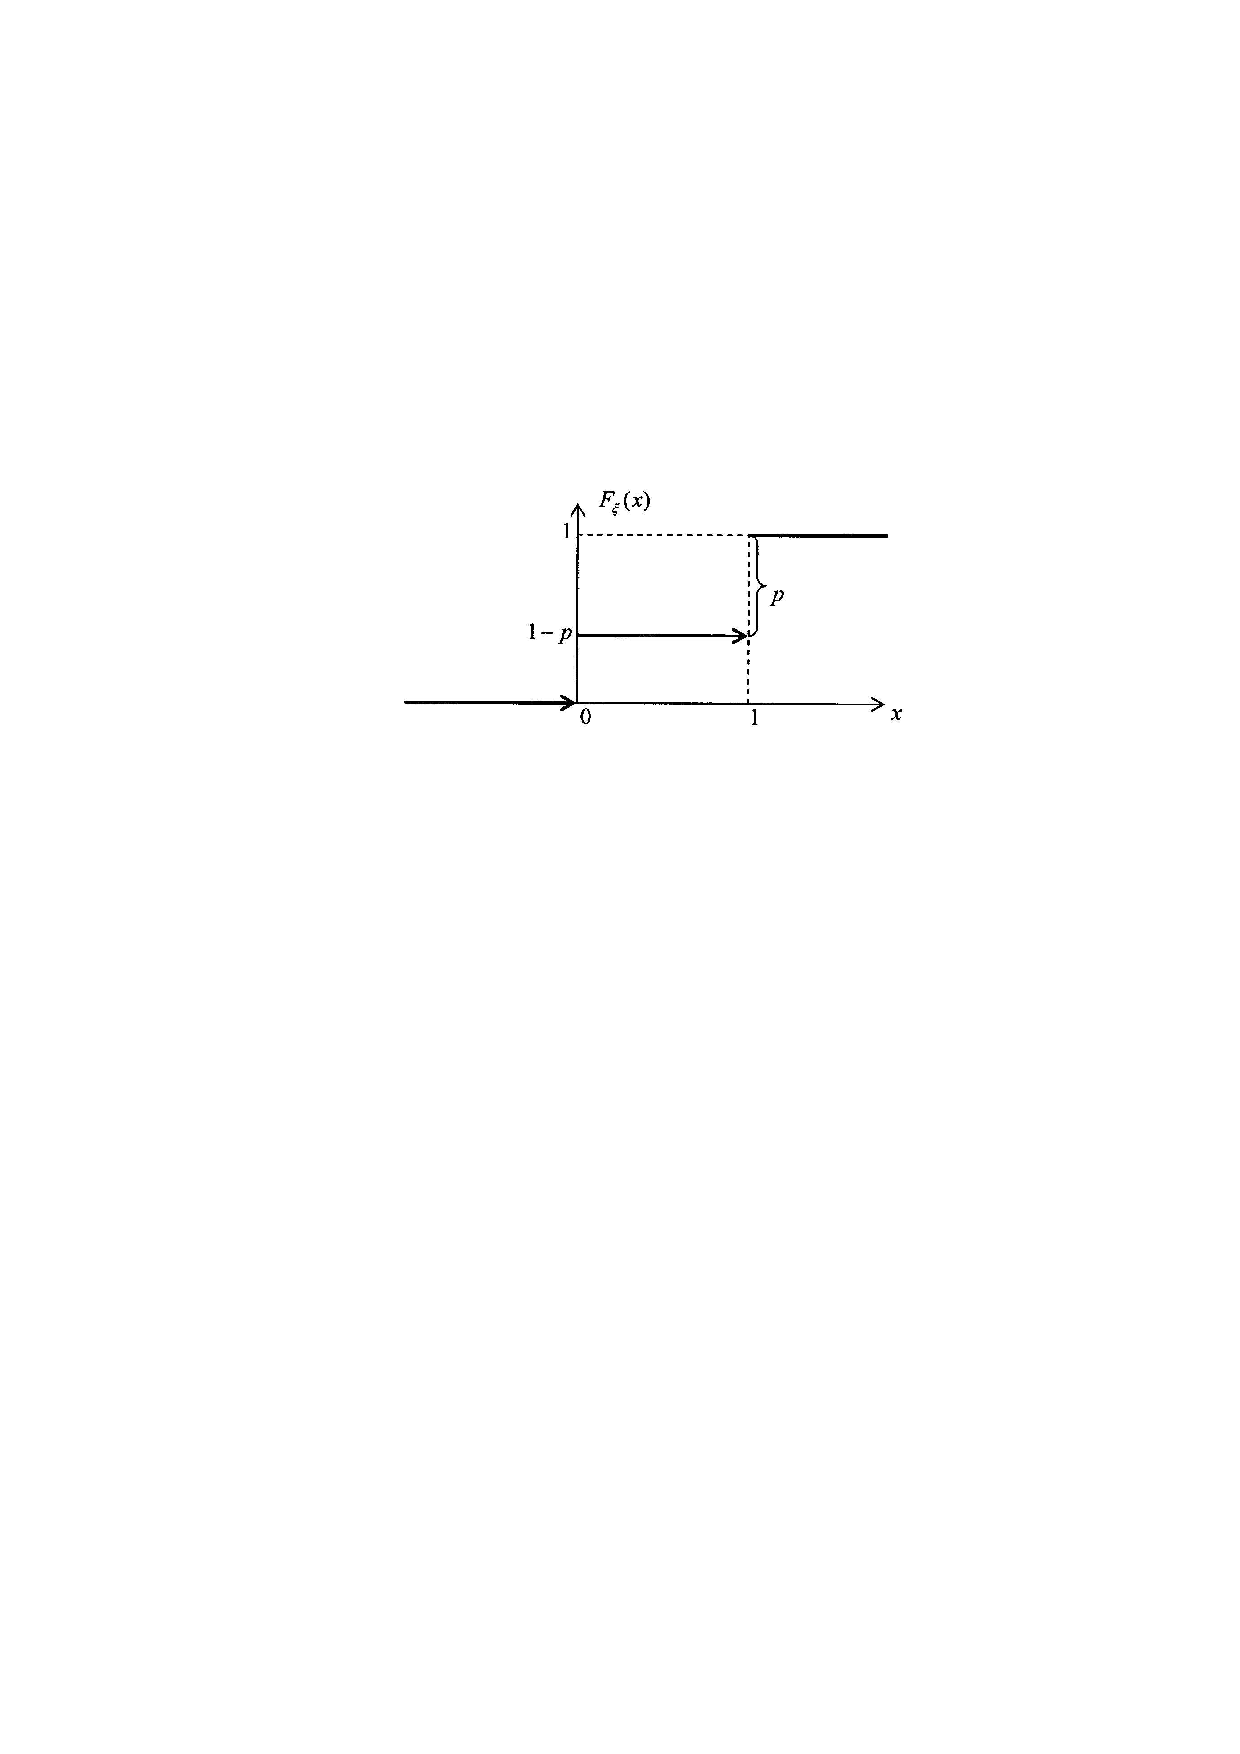
\includegraphics[]{pic/pic10}
	\caption{Функция распределения Бернулли.}
	\label{fig10}
\end{figure}

3) Случайная величина $\xi$ — номер грани при подбрасывании игральной
кости имеет функцию распределения, показанную на рис. \ref{fig11}.
\begin{figure}[H]
	\centering
	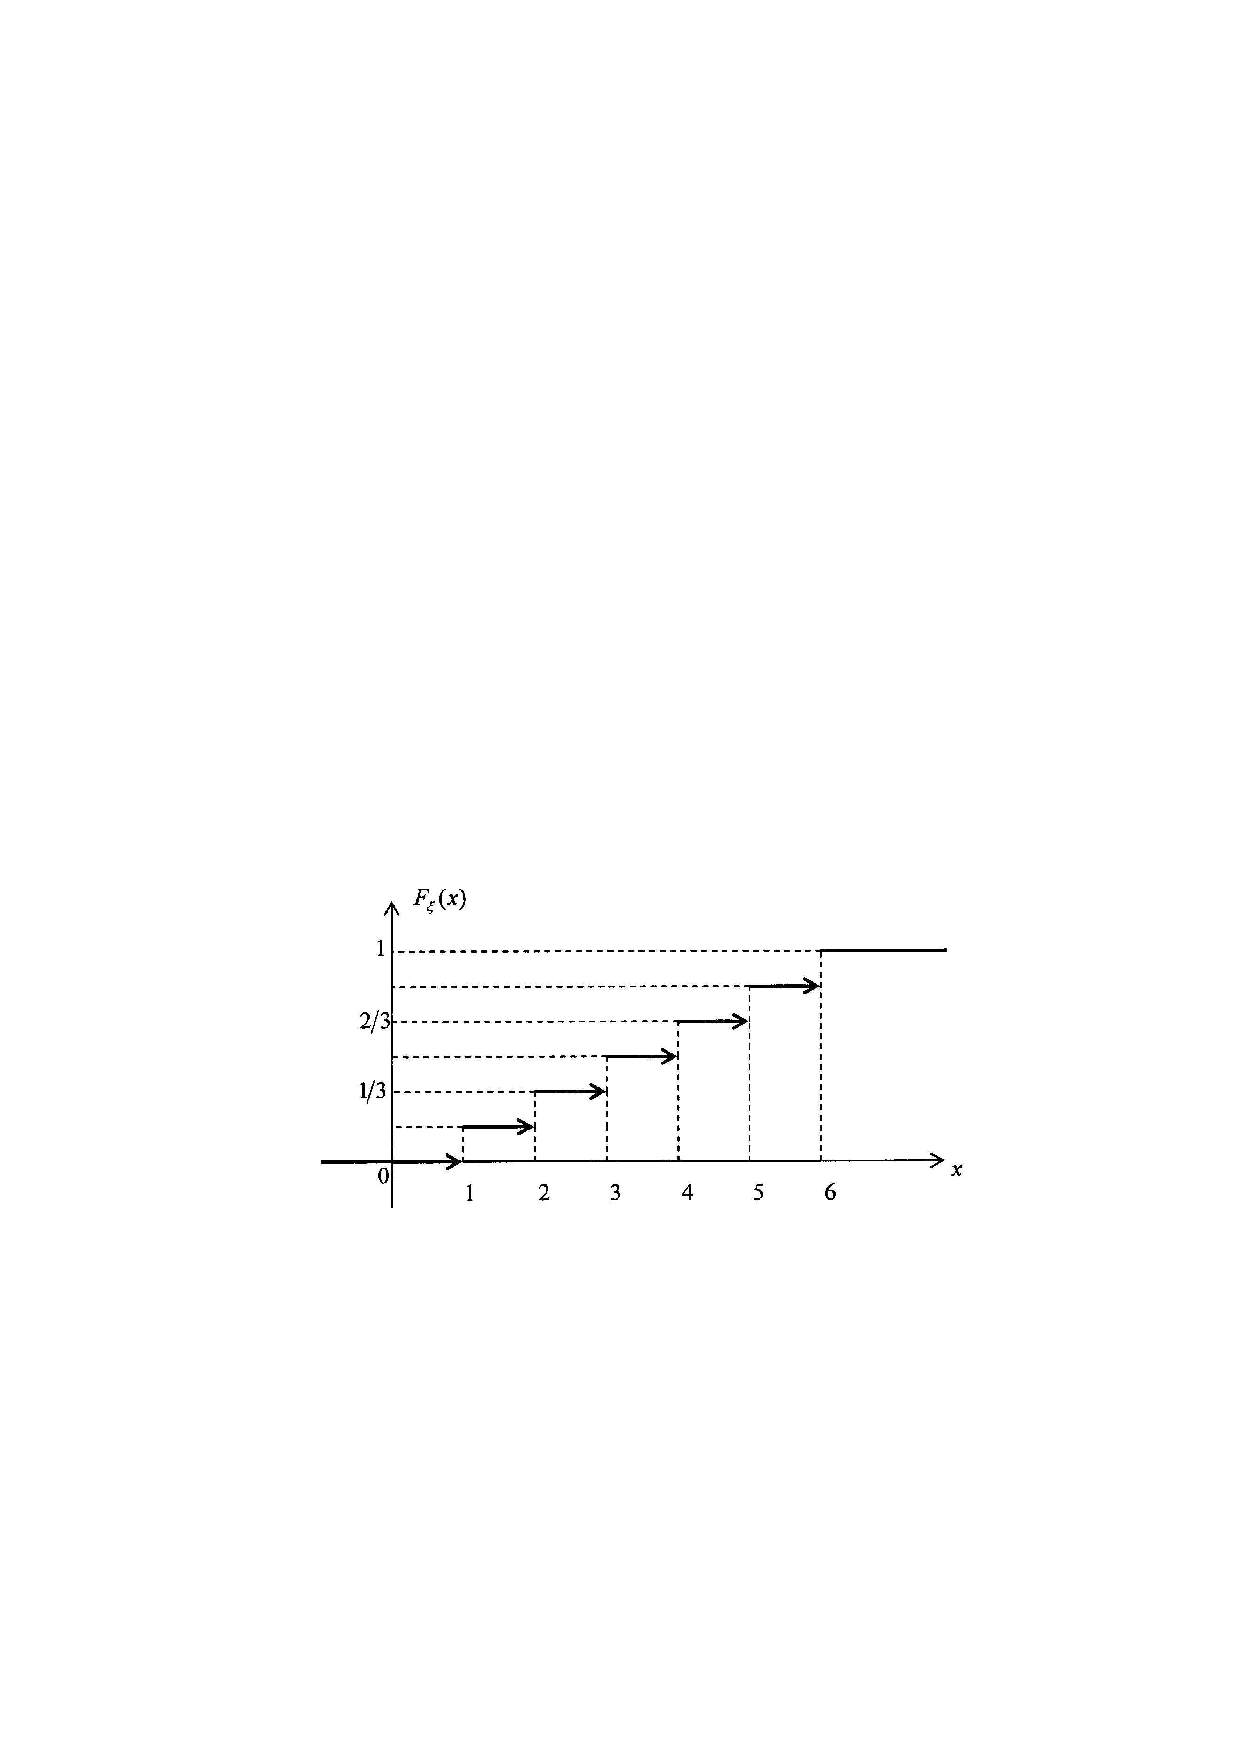
\includegraphics[]{pic/pic11}
	\caption{Функция распределения выпадения числа на игральной кости.}
	\label{fig11}
\end{figure}

4) Случайная величина $\xi$ — номер появления успеха в геометрическом
распределения имеет ряд распределения 
\begin{tabular}{|c|c|c|c|c|c|}
\hline
$\xi$ & $1$ & $2$ & $\dots$ & $k$ & $\dots$\\ \hline
$\P$ & $p$ & $pq$ & $\dots$ & $pq^{k-1}$ & $\dots$\\ \hline
\end{tabular}
и имеет функцию распределения, показанную на рис. \ref{fig12}.
В дальнейшем мы будем использовать следующие обозначения для пределов функций слева и справа соответственно:
\begin{gather*}
	\lim_{\varepsilon\to 0}h(x-\epsilon)\stackrel{\text{опр}}{=}h(x-0) \,\, \text{и} \,\,
	\lim_{\varepsilon\to 0}h(x+\epsilon)\stackrel{\text{опр}}{=}h(x+0),
\end{gather*}
где всегда $\varepsilon >0$.

\begin{figure}[H]
	\centering
	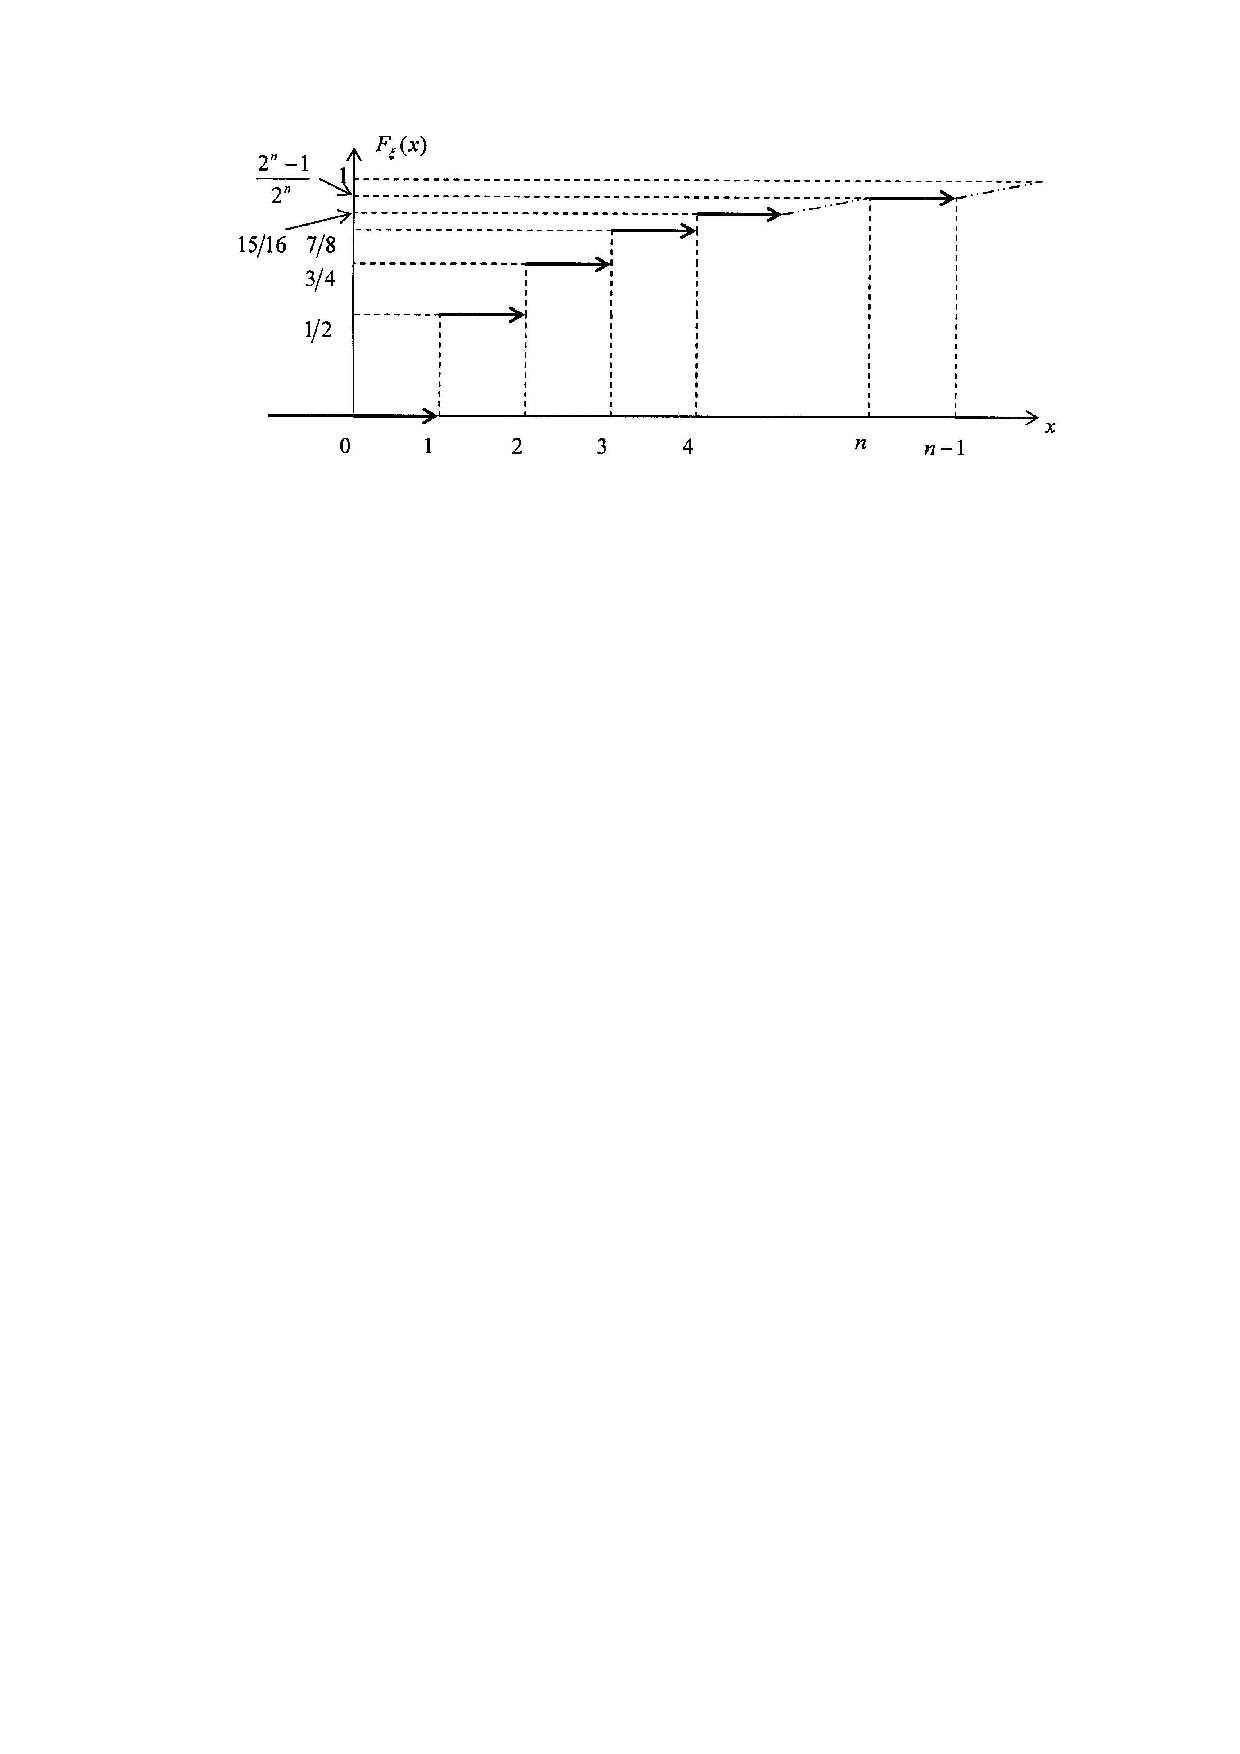
\includegraphics[]{pic/pic12}
	\caption{Функция распределения выпадения числа на игральной кости.}
	\label{fig12}
\end{figure}


Функция распределения $F_{\xi}(x)$ обладает следующими свойствами.

\begin{theorem}
\label{th:11.4}
% \newline
\vspace{1em}

	\begin{enumerate}

		\item $F_{\xi}(x)$ — неубывающая функция, другими словами,
			если $x_1 < x_2$, то $F_{\xi}(x_1) \leqslant F_{\xi}(x_)$.
		\item $F_{\xi}(-\infty)=\lim\limits_{x\to-\infty}F_{\xi}(x)=0$ и 
			$F_{\xi}(+\infty)=\lim\limits_{x\to+\infty}F_{\xi}(x)=1$
		\item $F_{\xi}(x)$ непрерывна справа: для любой точки $x_0 \in \mathbb{R}$ имеем $$F_{\xi}(x+x_0) =F_{\xi}(x_0)$$
	\end{enumerate}
\end{theorem}

\begin{proof}
	По пп. \ref{def:11.3}, \ref{lemma:3.3}, \ref{def:3.1} имеем  
	\begin{enumerate}
		\item $F_{\xi}(x_2)-F_{\xi}(x_1)=\P(\xi\leqslant x_2)-\P(\xi\leqslant x_1)=
			\P\{\xi\leqslant x_2\}\ssm \P\{\xi\leqslant x_1\}= \\
			=\P(x_1<\xi\leqslant x_2)\geqslant 0$.
		
		\item $F_{\xi}(-\infty)=\lim\limits_{x\to-\infty}F_{\xi}(x)=\lim\limits_{x\to-\infty}\P(\xi\leqslant x)=\P(\xi\leqslant-\infty)=0$ \, и \,
		$F_{\xi}(+\infty)=\lim\limits_{x\to+\infty}F_{\xi}(x)=\lim\limits_{x\to+\infty}\P(\xi\leqslant x)=\P(\xi\leqslant+\infty)=1$.
		
		\item $F_{\xi}(x_0+0)=\lim\limits_{\varepsilon\to 0}F_{\xi}(x_0+\varepsilon)=\lim\limits_{x\to\varepsilon}\P(\xi\leqslant x_0+\varepsilon)=\P(\xi\leqslant x_0)=F_{\xi}(x_0)$.
		
	\end{enumerate}

\end{proof}

\begin{theorem}
\label{th:11.5}
	Функция распределения имеет не более чем счётное мно-
жество скачков.
\end{theorem}

\begin{proof}
	Разобьём множество H всех скачков на подмножества скач-
ков по убыванию высоты h:
	
	1) $H_1$ – множество скачков высоты $h\in(\frac{1}{2},1]$,

	2)  $H_2$ – множество скачков высоты $h\in(\frac{1}{4},\frac{1}{2}]$,

	3) $H_2$ – множество скачков высоты $h\in(\frac{1}{8},\frac{1}{4}]$,

	\dots

	$n)$ – множество скачков высоты $h\in(\frac{1}{2^n},\frac{1}{2^{n-1}}]$

	\dots



Видно, что множества $H_n$ для всех $n\in\mathbb{Z}$ попарно непересекающиеся, т.е.
$H_i \cap H_j=\O$  при $i\neq j$; и $\bigcup\limits_{i=1}^{\infty}=H$.
Функция распределения может иметь

Во-первых, 	не более одного  скачка высоты $h\in(\frac{1}{2},1]$,т.е. 
$\mu(H_1)\leqslant 1$;

Во-вторых, 	не более трёх  скачков высоты $h\in(\frac{1}{4},\frac{1}{2}]$,т.е. 
$\mu(H_2)\leqslant 3$;

В-третьих, 	не более семи  скачков высоты $h\in(\frac{1}{8},\frac{1}{4}]$,т.е. 
$\mu(H_3)\leqslant 7$;

\ldots

В-n-ых, не более $2^n-1$ скачков высоты $h\in(\frac{1}{2^n},\frac{1}{2^{n-1}}]$,т.е.
$\mu(H_n)\leqslant 2^n-1$;

\ldots

Можно занумеровать все скачки по убыванию их высоты, нумеруя при
этом скачки равной высоты, если такие повстречаются. Эта нумерация ставит
множество всех скачков во взаимно однозначное соответствие с множеством
$\mathbb{Z}$ натуральных чисел. Что и требовалось доказать.

\end{proof}

\begin{theorem}[О связи вероятности событий-интервалов с функцией
распределения]
\label{th:11.6}
	Для любых точек $x,a,b \in\mathbb{R}$, где $a<b$, имеем 
	\newline
	\begin{enumerate}
		\item $\P(\xi<x)=F_{\xi}(x-0)$,
		\item $\P(\xi=x)=F_{\xi}(x)-F_{\xi}(x-0)$,
		\item если $F_{\xi}$ непрерывна в точке x, то $\P(\xi = x) = 0$;
		\item  $\P(a<\xi\leqslant b)=F_{\xi}(b)-F_{\xi}(a)$,
		\item $\P(a\leqslant\xi\leqslant b)=F_{\xi}(b)-F_{\xi}(a-0)$,
		\item $\P(a<\xi<b)=F_{\xi}(b-0)-F_{\xi}(a)$
		\item $\P(a\leqslant\xi<b)=F_{\xi}(b-0)-F_{\xi}(a-0)$.
	\end{enumerate}
\end{theorem}

\begin{proof}
	\begin{enumerate}
		\item $\P(\xi<x)=\lim\limits_{\varepsilon\to 0} \P(\xi\leqslant x-\varepsilon)=
		\lim\limits_{\varepsilon\to 0} F_{\xi}(x-\varepsilon)=F_{\xi}(x-0)$.

		\item $\P(\xi=x)=\P(\{\xi\leqslant x\})\ssm\{\xi<x \})=\P(\xi\leqslant x)-\P(\xi<x)=F_{\xi}(x)-F_{\xi}(x)$.

		\item $\P(\xi=x)=F_{\xi}-F_{\xi}(x-0)=F_{\xi}(x)-\lim\limits_{\varepsilon\to 0} F_{\xi}(x-\varepsilon)=F_{\xi}(x)-F_{\xi}(x)=0.$

		\item $\P(a<\xi\leqslant b)= \P(\{\xi\leqslant b \})\ssm \{\xi\leqslant a \}=
		\P(\xi\leqslant b)-\P(\xi\leqslant a)= F_{\xi}(b)-F_{\xi}(a).$

		\item Самостоятельно

		\item Самостоятельно

		\item Самостоятельно
	\end{enumerate}
\end{proof}

\begin{consq}
\label{consq:11.7}
	Если функция распределения $F_{\xi}(x)$ непрерывна, то 
	\begin{gather*}
		\P(a\leqslant \xi<b)=\P(a<\xi<b)=\P(a\leqslant \xi \leqslant b)= \P(a< \xi\leqslant b)= \\ 
		=F_{\xi}(b)-F_{\xi}(a).
	\end{gather*}
\end{consq}